% Chapter 3 from the thesis template file
%   that contains an example table and figure.

%Chapter 3: Background
%1) Introduction paragraph summarizing the flow/content/structure of the Background chapter
%2) Radiometer Basics
%	a) Power Detection
%	b) Integration and filtering
%	c) Metrics
%		i) Sensitivity
%		ii) Stability
%	d) Implementation
%3) Software Defined Radio Basics
%	a) High-level figure of the components of a generic SDR.
%	b) SDR Operation
%	c) GNURadio Operation
%4) Software Defined Radio Development Platform (i.e. your specific platform)
%	a) Hardware (i.e. N200)
%	b) Software (i.e. GNU Radio)  

\chapter{BACKGROUND}\label{ch:background}
This chapter gives background information on the operation of  traditional radiometers and on software defined radios.  We begin by looking at the major components of a radiometer and how it measures power.  Next the metrics used to measure the performance of a traditional radiometer are discussed.  Then an overview of how software defined radios operate is given.  Finally, we review the tools used to develop a software defined radio based radiometer.  

%We begin with an overview of a traditional radiometer and how this type of radiometer works.  This is followed by high level examination of a software defined radio.  Finally we will discuss the hardware and software to be used for our development of a software defined radiometer.

\section{Radiometer Basics}\label{rad_basics}
A radiometer is a device designed to measure thermal electromagnetic emission by a material media due to the electron agitation within the material.[\cite{ulaby}.  This electromagnetic emission is the thermal noise of the object and can be correlated to the physical temperature of the object[\cite{Nyquist1928thermal}].  Because of this correlation, the amount of noise received is called the noise temperature and it is measured in Kelvin. 

There are six stages common to all radiometers.  They are:

\begin{enumerate}
\item Source (antenna or $T_{A}$)
\item Bandwidth ($\beta$),
\item Amplification (Gain or $G$),
\item Power detection ($X^{2}$),
\item Integration ($\tau$),
\item Output (Voltage, rQ or Kelvin).
\end{enumerate}

Figure \ref{trad_radiometer} illustrates how a signal propagates through a radiometer.  First, the signal from the source enters the antenna, $T_A$.  Next the signal is filtered to a set bandwidth, $\beta$.  This filtered signal is then amplified by Low Noise Amplifiers (LNAs) by a gain of $G$.  The power information is then extracted from the signal using a square-law detector, $X^2$.  A square-law detector takes the input RF signal and produces a voltage that is proportional to the square of the voltage[\cite{Leinweber}].  This voltage output from the square-law detector is then integrated to smooth the signal using an integration time of $\tau$.  Finally the integrated voltage signal is then measured.

A non-physical object that is present in all radiometers is system noise, represented as $T_{N}$.  System noise is noise that is generated from within the radiometer due to thermal agitation.  A radiometer is designed to reduce the system noise as much as possible by using low-loss components and amplifiers that are low noise such as Low Noise Amplifiers (LNA). 

{\begin{figure}[h!tb] 
\centering
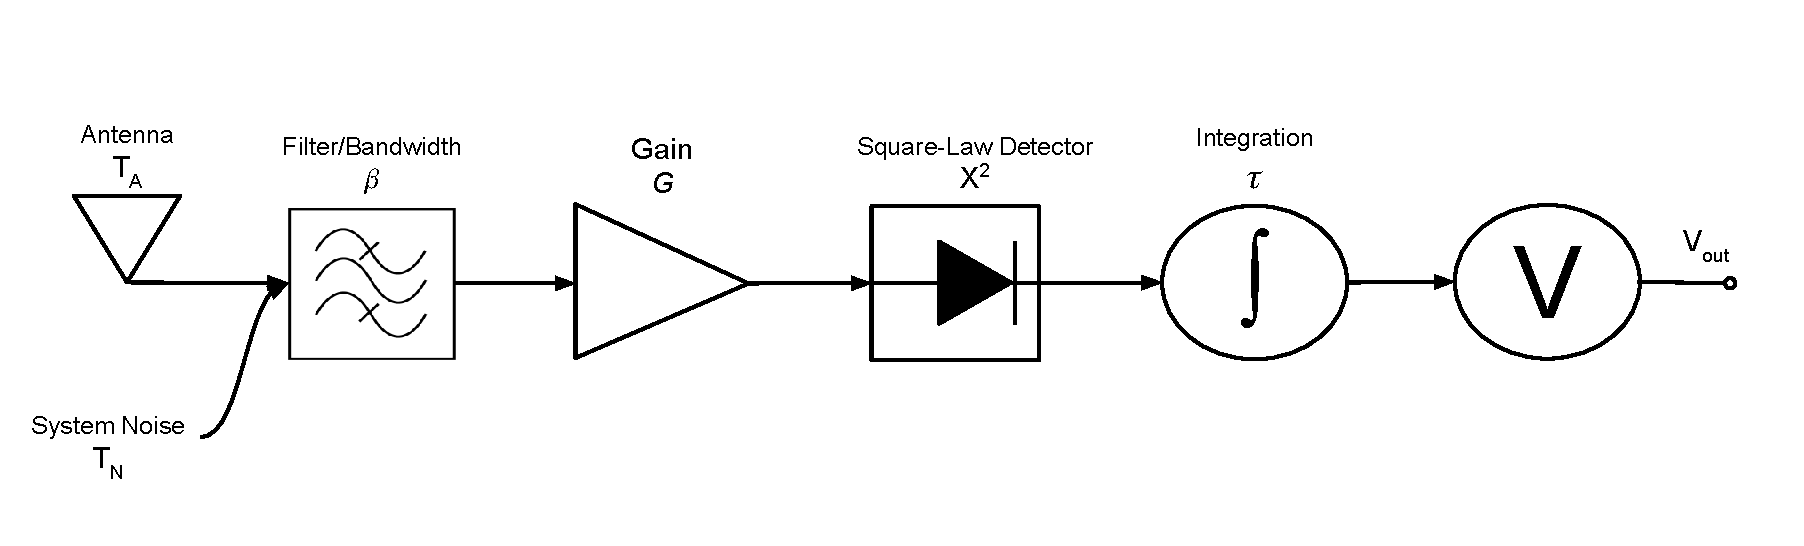
\includegraphics[width=\textwidth]{Images/Traditional_Radiometer.pdf}
\isucaption{A total power radiometer block diagram}
\label{trad_radiometer}
\end{figure}
}

\subsection{Power Measurement}\label{pwr_measurement}

As shown in Equation \ref{eq:power_rad_eq}, the power measured by an ideal radiometer is equal to the product of the power received from the source ($T_A$), the gain ($G$) and the bandwidth ($\beta$) of the radiometer, and the Boltzmann constant ($k=1.38 x 10^{-23} J/K$).

\begin{equation} \label{eq:power_rad_eq}
P=k*\beta*G*(T_{A}) (watts)
\end{equation}

%\begin{equation} \label{eq:boltzmann}
%k = 1.38 x 10^{-23} J/K
%\end{equation}

While the components of an ideal radiometer do not contribute noise power ($T_N$) to the system, they do in a real radiometer.  The impact of this internally generated and unwanted noise on the power measured by the radiometer is captured by Equation \ref{eq:final_power}.

\begin{equation} \label{eq:final_power}
P=k*\beta*G*(T_{A}+T_{N}) watts
\end{equation}

Gain ($G$) and bandwidth ($\beta$) are important design parameters of a radiometer.  While a large gain is desired to amplify the source signal, the magnitude of the gain must be limited since it also amplifies the unwanted system noise ($T_N$).

Since the bandwidth of the source signal is typically wide (ideally infinite), ideally one wants the radiometers bandwidth to be wide (large) as well.  The two primary limiting factors are: 1) hardware limitations (e.g. LNA operating limits), and 2) unwanted signals located at a number of frequencies (e.g. radio communication signals).

\emph{Low Noise Amplification.}  The method used by most radiometer to mitigate the system noise contributed during the signal amplification is daisy chaining devices called Low Noise Amplifiers (LNAs).  The total amount of amplification we can expect from $N$ LNAs, is the sum of the gain values of each LNA shown in equation \ref{gain_sum}.

\begin{equation}\label{gain_sum}
G_{total}=G_1 + G_2 + G_3 + \cdots +G_{n-1}
\end{equation}

A performance metric of a LNA is the noise figure ($NF$).  The noise figure gives us the difference between the actual noise output and an ideal amplifier with the same gain and bandwidth attached to a matched load at the standard noise temperature (290 K).

Another terminology used is the noise factor ($F$).  The noise factor shows how much the signal to noise ratio is degraded by the LNA.  The noise factor is related to the noise figure shown in equation \ref{noise_figure}.

\begin{equation}\label{noise_figure}
NF=10 * \log_{10}(F) dB
\end{equation}

For devices that are cascaded, the total noise factor is found by the Friis formula and results in equation \ref{noise_factor}.  This equation allows us to examine how the noise figure, and also the noise factor propagates through the cascaded LNAs.  

\begin{equation}\label{noise_factor}
F=F_1+\frac{F_2-1}{G_1}+\frac{F_3-1}{G_1 G_2}+\frac{F_4-1}{G_1 G_2 G_3}+\cdots +\frac{F_n-1}{G_1 G_2 G_3 \cdots G_{n-1}}
\end{equation}

The key implication of this property is that the first LNA in the cascade contributes the most system noise.  As a consequence, it is critical that the first LNA has the smallest noise factor , while the remaining LNAs provide a majority of the signal gain.  While these LNAs provide higher gain they will have higher noise figures, but their contribution to the overall system noise is a fraction of the first LNA.

\subsection{Radiometer Performance Metrics}\label{performance_metrics}

Two criteria used to determine how well a radiometer performs are: 1) Sensitivity and 2) Stability.  These criteria determine the smallest change in signal noise temperature (i.e. power) the radiometer can detect, and the amount drift power measurements have over an extended period of time.

\emph{Sensitivity}.  Sensitivity of a radiometer is the smallest change in power that can be detected.  A radiometer must be able to differentiate between signal noise received by  the antenna ($T_{A}$) and the system generated noise ($T_N$).

Two methods to quantify the sensitivity of a radiometer are: 1) experimentally, and 2) analytically.  Experimentally, sensitivity can be computed as the standard deviation of the measured power (assuming a stable radiometer).  Analytically, sensitivity can be computed as a function of radiometer properties.  Equation \ref{NEAT_EQ} gives this relation.  The term Noise Equivalent Delta ($\Delta$) Temperature ($NE\Delta T$) is often used interchangeably with sensitivity.  As can be seen in Equation \ref{NEAT_EQ}, sensitivity improves (i.e. becomes smaller) as the bandwidth ($\beta$) and integration time ($\tau$) of the radiometer increases[\cite{ulaby}].

\begin{equation} \label{NEAT_EQ}
NE\Delta T=\frac{T_{A}+T_{N}}{\sqrt{\beta * \tau}} 
\end{equation}

The following example illustrates the impact system generated noise has on a radiometers ability to detect changes in signal noise.  Lets assume we want a sensitivity of 1 K.  If there is no system generated noise (i.e. $T_N = 0$) and the received signal at the antenna is 200 K (i.e. $T_A = 200$), we can then calculate our receiver sensitivity by using equation \ref{NEAT_EQ}.  Lets assume a bandwidth of 10 MHz (i.e. $\beta = 10 x 10^6$) and that our integration time is 40 milliseconds (i.e. $\tau = 0.04$).  We can now take these values and put them in Equation \ref{NEAT_EQ} which results in Equation \ref{NEAT_EX1}.

\begin{equation} \label{NEAT_EX1}
NE\Delta T=\frac{200 + 0}{\sqrt{10 x 10^6 * 0.04} = 1 K} 
\end{equation}

Equation \ref{NEAT_EX1} gives us a result of 1 K for our sensitivity which meets our goal.  Because we do not have an ideal radiometer (i.e. $T_N != 0$) lets assume our system noise added is 800 K (i.e. $T_N = 800$).  Assuming that our bandwidth ($\beta$), our integration time ($\tau$) and our antenna signal ($T_A$) is the same, we can now apply Equation \ref{NEAT_EQ} which results in Equation \ref{NEAT_EX2}.  This results in a sensitivity of 5 K, which is five times higher than our ideal sensitivity of 1 K. 

\begin{equation} \label{NEAT_EX2}
NE\Delta T=\frac{200 + 800}{\sqrt{10 x 10^6 * 0.04} = 5 K} 
\end{equation}

As can be clearly seen, system noise makes the job of detecting changes in signal noise more difficult[\cite{skou}].

Section \ref{Exp2_analysis} uses these two methods of finding sensitivity as a cross validation of the correctness of a SDR based radiometer.

%To understand this, look at the example of where T$_{A}$ has a value of 200 K and T$_{N}$ has a value of 800 K.  Since T$_{N}$ is added to the antenna signal, we have a total noise temperature of 1,000 K.  This means to detect a change as small as 1 K, the difference between 1,000 K and 1,001 K needs to be measured.[\cite{skou}].

%The ability of a radiometer to detect these small changes is the radiometer's sensitivity, or the standard deviation of the output signal from the radiometer.  This sensitivity is also referred to as the Noise Equivalent Delta ($\Delta$) Temperature or NE$\Delta$T and is shown in equation \ref{NEAT_EQ}. 

%\begin{equation} \label{NEAT_EQ}
%NE\Delta T=\frac{T_{A}+T_{N}}{\sqrt{\beta * \tau}} 
%\end{equation}

%The sensitivity of the radiometer is a function of the bandwidth, ($\beta$), of the incoming signal and the integration time, ($\tau$) used.  Since the sensitivity improves as the bandwidth increases, as much bandwidth that is possible is desired.  In a traditional radiometer, this bandwidth is often fixed and it is dependent on the band-pass filters used in the radiometer.  A longer integration time ($\tau$) will also help improve the sensitivity of the radiometer to a certain degree.[\cite{ulaby}]

\emph{Stability.}  Stability for a radiometer means that any fluctuations we see is a result of the source and not a change occurring within the radiometer.  Lets examine Equation \ref{eq:final_power} which defines the total power the radiometer receives.  If our bandwidth ($\beta$), Gain ($G$), system noise ($T_N$), and Boltzmann constant ($k$) are constant, then the system is stable.  We can assume that our bandwidth is fixed and that our system noise is constant.  This results in our Gain ($G$) being the uncertain variable that may cause unwanted fluctuations[\cite{Evans}]. 

Radiometer instabilities are due to Low Noise Amplifier (LNAs) gain fluctuations.  Two factors cause gain these gain fluctuations: 1) fluctuations in the LNA's voltage supply, and 2) fluctuation in the LNA's physical temperature.  

The impact these gain fluctuations have on stability is given by equation \ref{eq:rad_stability}.  Where:

\begin{itemize}
\item $\Delta T_G$ is the noise temperature fluctuation,
\item $\Delta G$ is the LNA gain fluctuation,
\item $G$ is the gain of the LNA and,
\item $T_{sys}$ is the combined antenna source ($T_A$) and system noise ($T_N$).
\end{itemize}

%Here, the change in the noise temperature due to gain fluctuations, $\Delta T_{G}$, is a result of the change in the gain, $\Delta G$ divided by our gain, $G$, and multiplied by our system noise, $T_{sys}$.  

\begin{equation} \label{eq:rad_stability}
\Delta T_G=T_{sys} \left(\frac{\Delta G}{G}\right)
\end{equation}

These gain fluctuations can be controlled by closely monitoring and controlling both the voltage and temperature of the LNAs. However, this adds levels of complexity to the radiometer, that may be impractical in some cases.  As an alternative, modifications to the basic radiometer given in Figure \ref{trad_radiometer} have been developed to compensate for these fluctuations.  There are three common types of radiometers designed to account for gain fluctuations.  They are: Dicke, Noise injection, and Polarimetric or Correlating radiometers.

\emph{Dicke Radiometer.}  Figure \ref{dicke_radiometer} shows the block diagram of a Dicke radiometer, which switches between the measurement of the source signal ($T_A$) and a known reference signal ($T_R$)[\cite{Dicke}].  By quickly switching between the source and reference signal at a frequency of $F_S$, a Dicke radiometer can reduce the impact of gain fluctuations on its stability.  

{\begin{figure}[h!tb] 
\centering
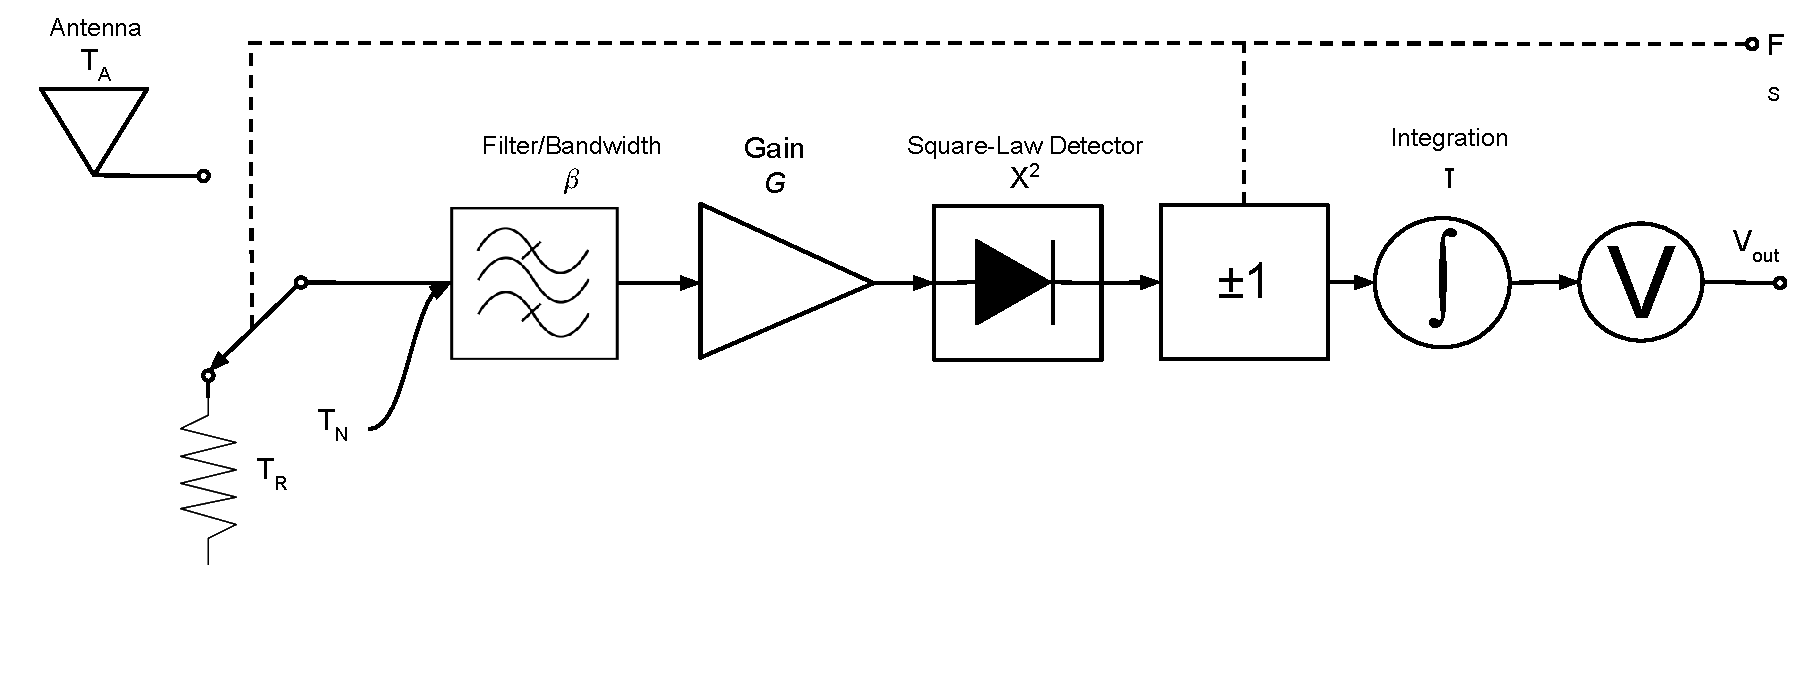
\includegraphics[width=\textwidth]{Images/Dicke_Radiometer.pdf}
\isucaption{A block diagram of a Dicke radiometer}
\label{dicke_radiometer}
\end{figure}
}

While a Dicke radiometer improves stability, it does so at the cost of not seeing the object of interest while it is measuring the reference signal.  This reduces the sensitivity of the radiometer since the source signal is only observed for a fraction of the time.

{\begin{figure}[h!tb] 
\centering
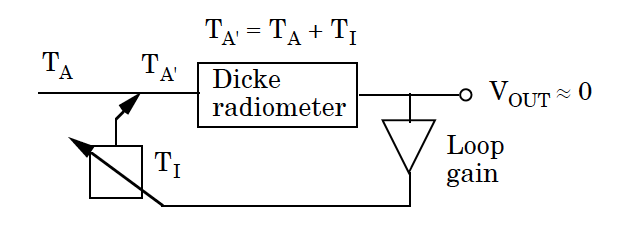
\includegraphics[width=\textwidth]{Images/NoiseInj_block.png}
\isucaption{A block diagram of a Noise Injection radiometer}
\label{NoiseInj_radiometer}
\end{figure}
}

\emph{Noise Injection Radiometer.}  A noise injection radiometer is a variation of the Dicke radiometer, where a variable noise signal ($T_I$) is injected into the RF chain as seen in Figure \ref{NoiseInj_radiometer}.  The injected noise signal power is adjusted so when added to the source signal, their sum equals to the reference signal.  This eliminates gain fluctuations, but increases system noise ($T_N$) which reduces radiometer sensitivity.

\emph{Polarimetric Radiometer} A polarimetric (or correlating) radiometer uses two polarized signals, referred to as vertically polarized (V-Pol) and horizontally polarized (H-Pol).  In order to accomplish this, an antenna with dual polarization is used [\cite{Fujimoto}].  Each polarized signal is fed into the radiometer and correlated.  Because the source noise signal has polarization and the gain fluctuations does not, the gain fluctuations can be eliminated.  This reduces gain fluctuations to increase stability, helping maintain sensitivity.  However, this is at the cost of increasing radiometer complexity and price, since two identical receivers (one for each polarization) is required. 


%Stability and accuracy are additional problems that need to be considered when looking at the radiometer system.  To begin we can once again look at the power received equation \ref{eq:final_power}.

%As we look at this equation, we can see that if $k$, $\beta$, $G$, and $T_{N}$ are constant, then stability can be assured.  The Boltzman constant $k$ is a known constant and we can also assume that our bandwidth, $\beta$, will also remain constant.  Gain and the noise temperature however will vary.  

 
\section{Software Defined Radios Basics} 
A Software Defined Radio (SDR) is a device that digitizes a received RF signal as soon as possible, and processes the digital representation of the signal using a computer, FPGA, or dedicated System on Chip (SoC).  A canonical software defined radio architecture consists of a power supply, antenna, analog to digital converter, and a processing unit to carry out radio functions in software [\cite{Mitola1995}]. An ideal software defined radio block diagram is shown in figure \ref{ideal_sdr}.

{\begin{figure}[h!tb] 
\centering
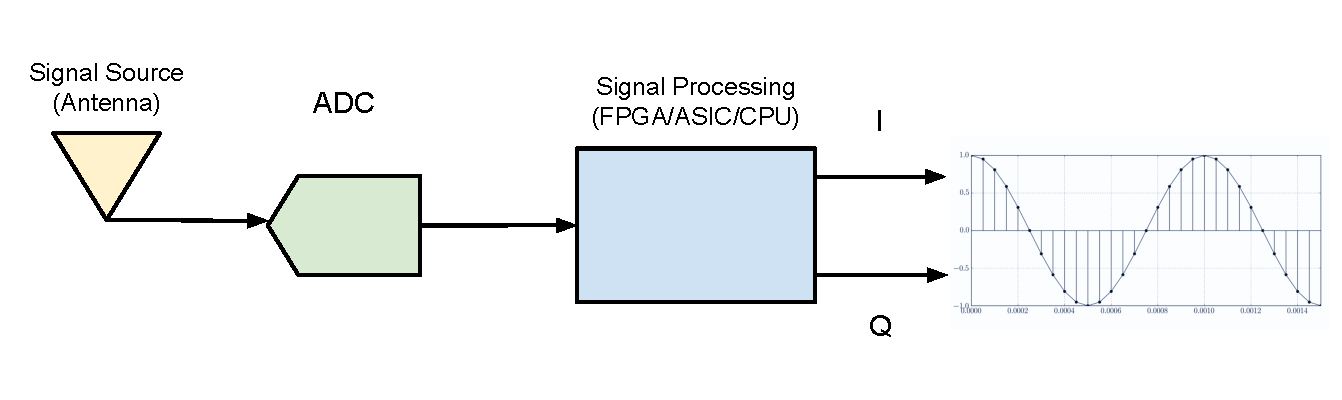
\includegraphics[width=\textwidth]{Images/SDR_Ideal_block.pdf}
\isucaption{An ideal software defined radio}
\label{ideal_sdr}
\end{figure}
}

A SDR can perform certain hardware functions in software (e.g. filtering).  This gives SDRs a high amount of flexibility because components that were normally performed in hardware can now be performed in software.  Changes can be made by simply uploading new software or firmware to the system.  This has a cost benefit as certain hardware components are no longer needed and changes made in software do not require additional hardware to be added, removed or modified.

A more realistic software defined radio is shown in figure \ref{prac_sdr}, where two items have been added.  First, an amplification of the signal (gain) is added to improve SDR sensitivity.  Second, a mixer is often used to down-convert the high frequency RF source signal to a lower frequency so a less expensive analog to digital converter can be used.  However, if the source signal frequency is already within the range of the analog to digital converter, then the mixer may be omitted.  

%An ideal software defined receiver simply has an antenna connected to an analog to digital converter which sends information to a processing unit such as a Field Programmable Gate Array (FPGA) or computer.  For a transmitter, we reverse it and use a digital to analog converter to produce the correct waveform which is then transmitted by the antenna.  In reality, SDRs require some additional hardware to make a viable working transceiver.  Amplification is still required to amplify the incoming signal and to amplify the signal going to the antenna.  Some SDRs also use a mixing stage to move a high frequency signal to a lower frequency signal.  This allows for less expensive analog to digital and digital to analog converters to be used.  

{\begin{figure}[h!tb] 
\centering
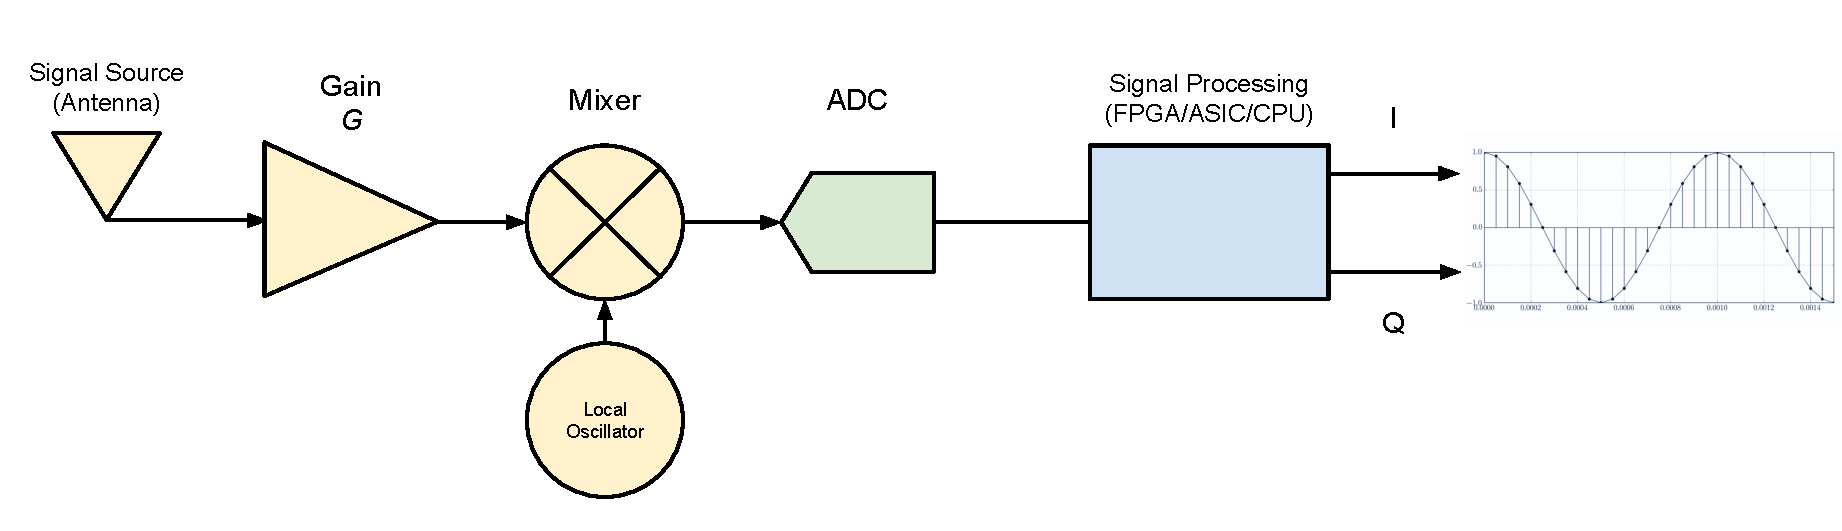
\includegraphics[width=\textwidth]{Images/SDR_Prac_block.pdf}
\isucaption{A typical software defined radio}
\label{prac_sdr}
\end{figure}
}

\emph{Software Defined Radio Applications.}  Software Defined Radios (SDRs) can be for a variety of applications, but have been primarly used in the area of communications.  Some examples of these applications include:  mobile communications, wireless local area networks, personal area networks and digital broadcast.  They appeal to applications where having the ability to change a modulation scheme or filter on the fly is desirable.  In these respects, SDRs often outperform traditional hardware-only radios because of their ability to easily change their operations through software.  

Early SDRs were expensive due to the cost of high speed analog to digital converters (ADCs) and high-end Field Programmable Gate Arrays (FPGA) that were required.  In recent years, the cost of SDRs have decreased due to the cost of these key components decreasing.  Also, while the cost of SDRs has gone down, their performance has increased.  This has led to SDRs becoming feasible for use in many new ways [\cite{jondral2005software}].


%But this is the strength of a software defined radio, it is capable of performing all of these operations and can be adapted to new ones by simply updating the software that defines it.

\section{Software Defined Radio Development Platform} \label{SDR_platform}
This section discusses the platform used to develop a software defined radio based radiometer.  The hardware and software tools used are off the shelf.  First, the hardware platform will be introduced, followed by the software platform.  

%The work of this thesis is to use an off the shelf software defined radio (SDR) to perform the same operation or better of a traditional analog radiometer.  Using a SDR radio also means that we are able to be more flexible in how the radiometer performs, is capable of frequency agility and adapting to changing conditions such as interference.  Using a software defined radio also allows for implementation of different radiometer types such as a correlation radiometer or a polarimetric radiometer that uses Stokes parameters [\cite{Wang}].  Normally, these require changes to hardware, but all of these types of radiometers can be implemented in software increasing the flexibility of the system.  

\subsection{Hardware Platform}
The hardware platform selected for this work is the Ettus Research Group N200 SDR shown in figure \ref{N200}.  The N200 has the following features that made it desirable for our specific application:

\begin{itemize}
\item Dual 14-bit ADC,
\item 25 MHz bandwidth per channel,
\item Modular daughter-board system for RF front end.
\end{itemize}

Its flexible architecture and ability to support a large bandwidth made the N200 an ideal hardware platform for the software defined radio based radiometer development.

{\begin{figure}[h!tb] 
\centering
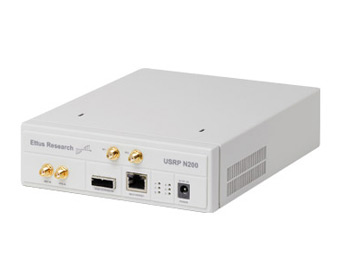
\includegraphics[width=7cm]{Images/n200}
\isucaption{The USRP N200 from Ettus Research (Image from Ettus Research Website - www.ettus.com)}
\label{N200}
\end{figure}
}

When selecting the hardware for this thesis, the requirements defined section \ref{requirements} were examined.  The bandwidth requirement was a deciding factor for hardware selection.  It was decided that a minimum bandwidth of 20 MHz was desired.  The 14-bit ADC was not a defined requirement, but was deemed to provide an adequate level of resolution.  The N200 has a flexible architecture through the use of daughter-boards.  

Figure \ref{N200_block} shows the overall architecture of the N200 SDR.  A daughter board directly receives the RF signal and then outputs analog I (in-phase) and Q (quadrature phase) signals that are then sampled by the N20014-bit  A/D converter.

{\begin{figure}[h!tb] 
\centering
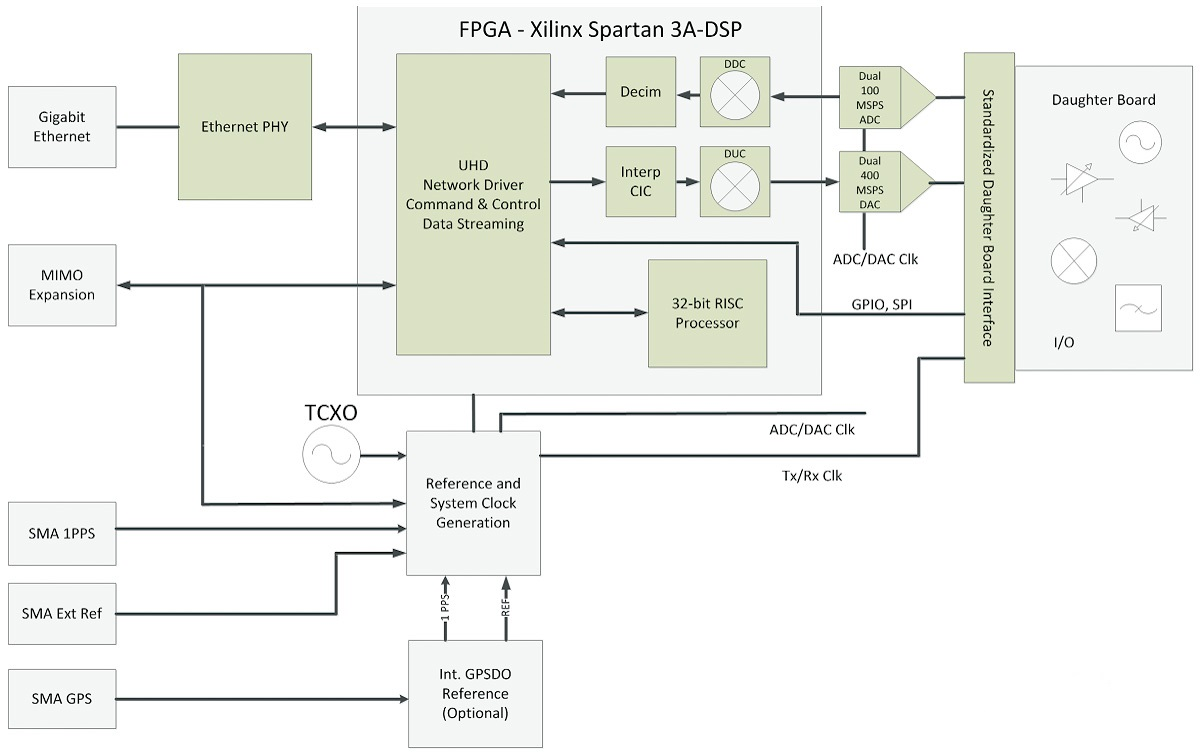
\includegraphics[width=14cm]{Images/n200_block_edited}
\isucaption{A block diagram of the Ettus N200 SDR. (Image from Ettus Research Website - www.ettus.com)}
\label{N200_block}
\end{figure}
}

%The requirements outlined above was the guiding factor in selecting the N200 SDR for our hardware platform.  These reasons, and the fact that this hardware is well supported by GNURadio, lead to using this for the work in this thesis.
%While not a defined requirement, it was indicated by Dr. Brian Hornbuckle that it would be ideal to look at two signals at the same time.  The N200 is able to have up to two daughter boards installed.

\emph{The DBSRX2 Receiver.}  The daughter board selected for this work was the DBSRX2 shown in figure \ref{dbsrx2}.  This daughter board is receive only, and operates between 800 MHz and 2400 MHz, which includes the frequency band required for this work (1400 MHz - 1425 MHz).

{\begin{figure}[h!tb] 
\centering
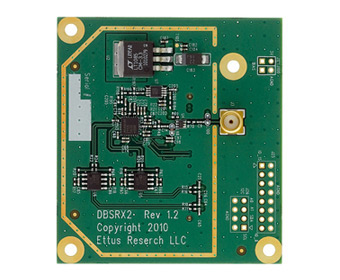
\includegraphics[width=7cm]{Images/dbsrx2.jpg}
\isucaption{The DBSRX2 daughter board from Ettus Research (Image from Ettus Research Website - www.ettus.com)}
\label{dbsrx2}
\end{figure}
}

The DBSRX2 has the RF hardware needed to transform the received RF signal into phase and quadrature phase outputs.  This includes a programmable gain amplifier, a direct-conversion converter, a mixer, and finally a band-pass filter.  Figure \ref{dbsrx2_block} provides a block diagram of the DBSRX2.  First, the signal received is amplified by the Programmable Gain Amplifier (PGA).  The PGA is can be configured by the software.  Next, the signal goes into a direct-conversion integrated circuit (a Maxim 2112).  This integrated circuit directly converts the RF signal into analog I (in-phase) and Q (quadrature phase) values and is composed of an integrated mixer and band-pass filter.

{\begin{figure}[h!tb] 
\centering
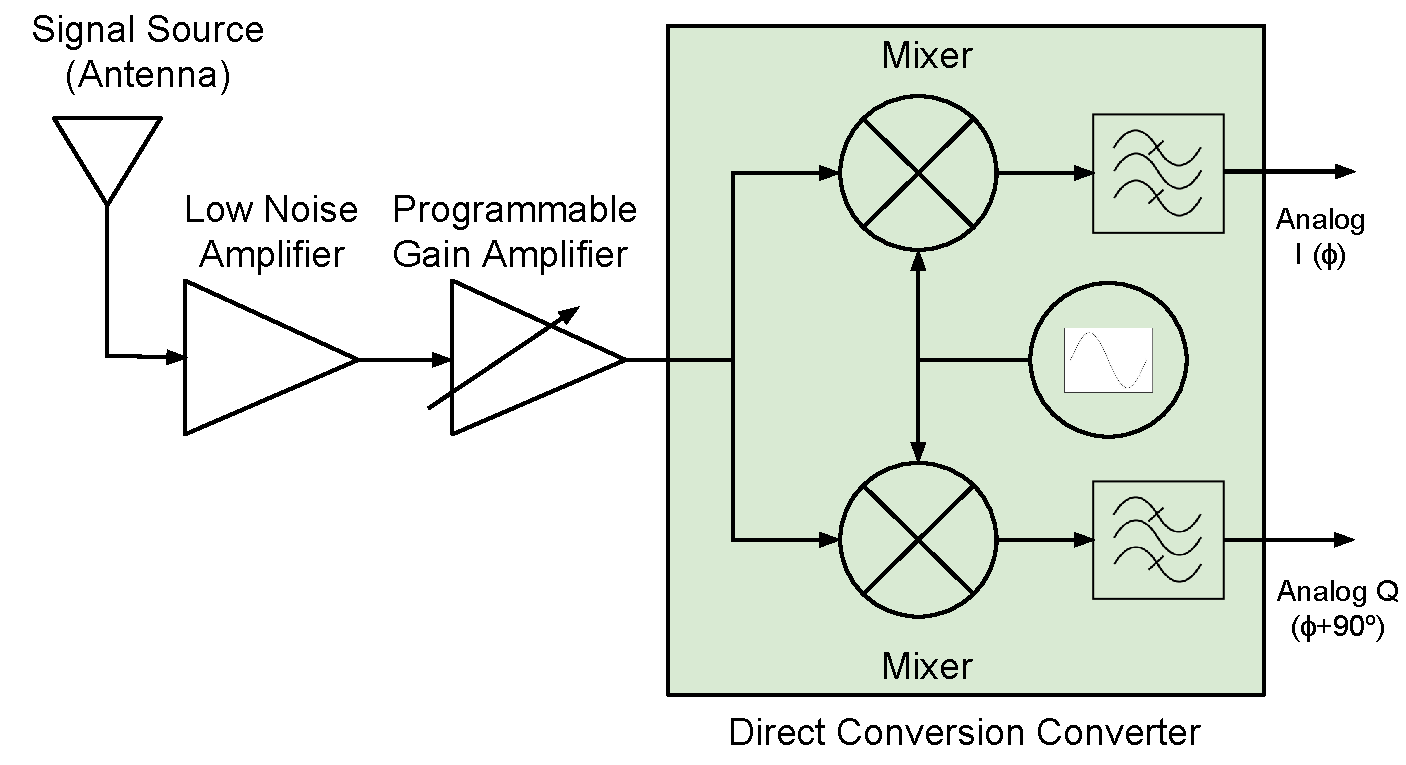
\includegraphics[width=12cm]{Images/DBSRX2_block.pdf}
\isucaption{Block diagram of the DBSRX2 daughter board.}
\label{dbsrx2_block}
\end{figure}
}

%{\begin{figure}[h!tb] 
%\centering
%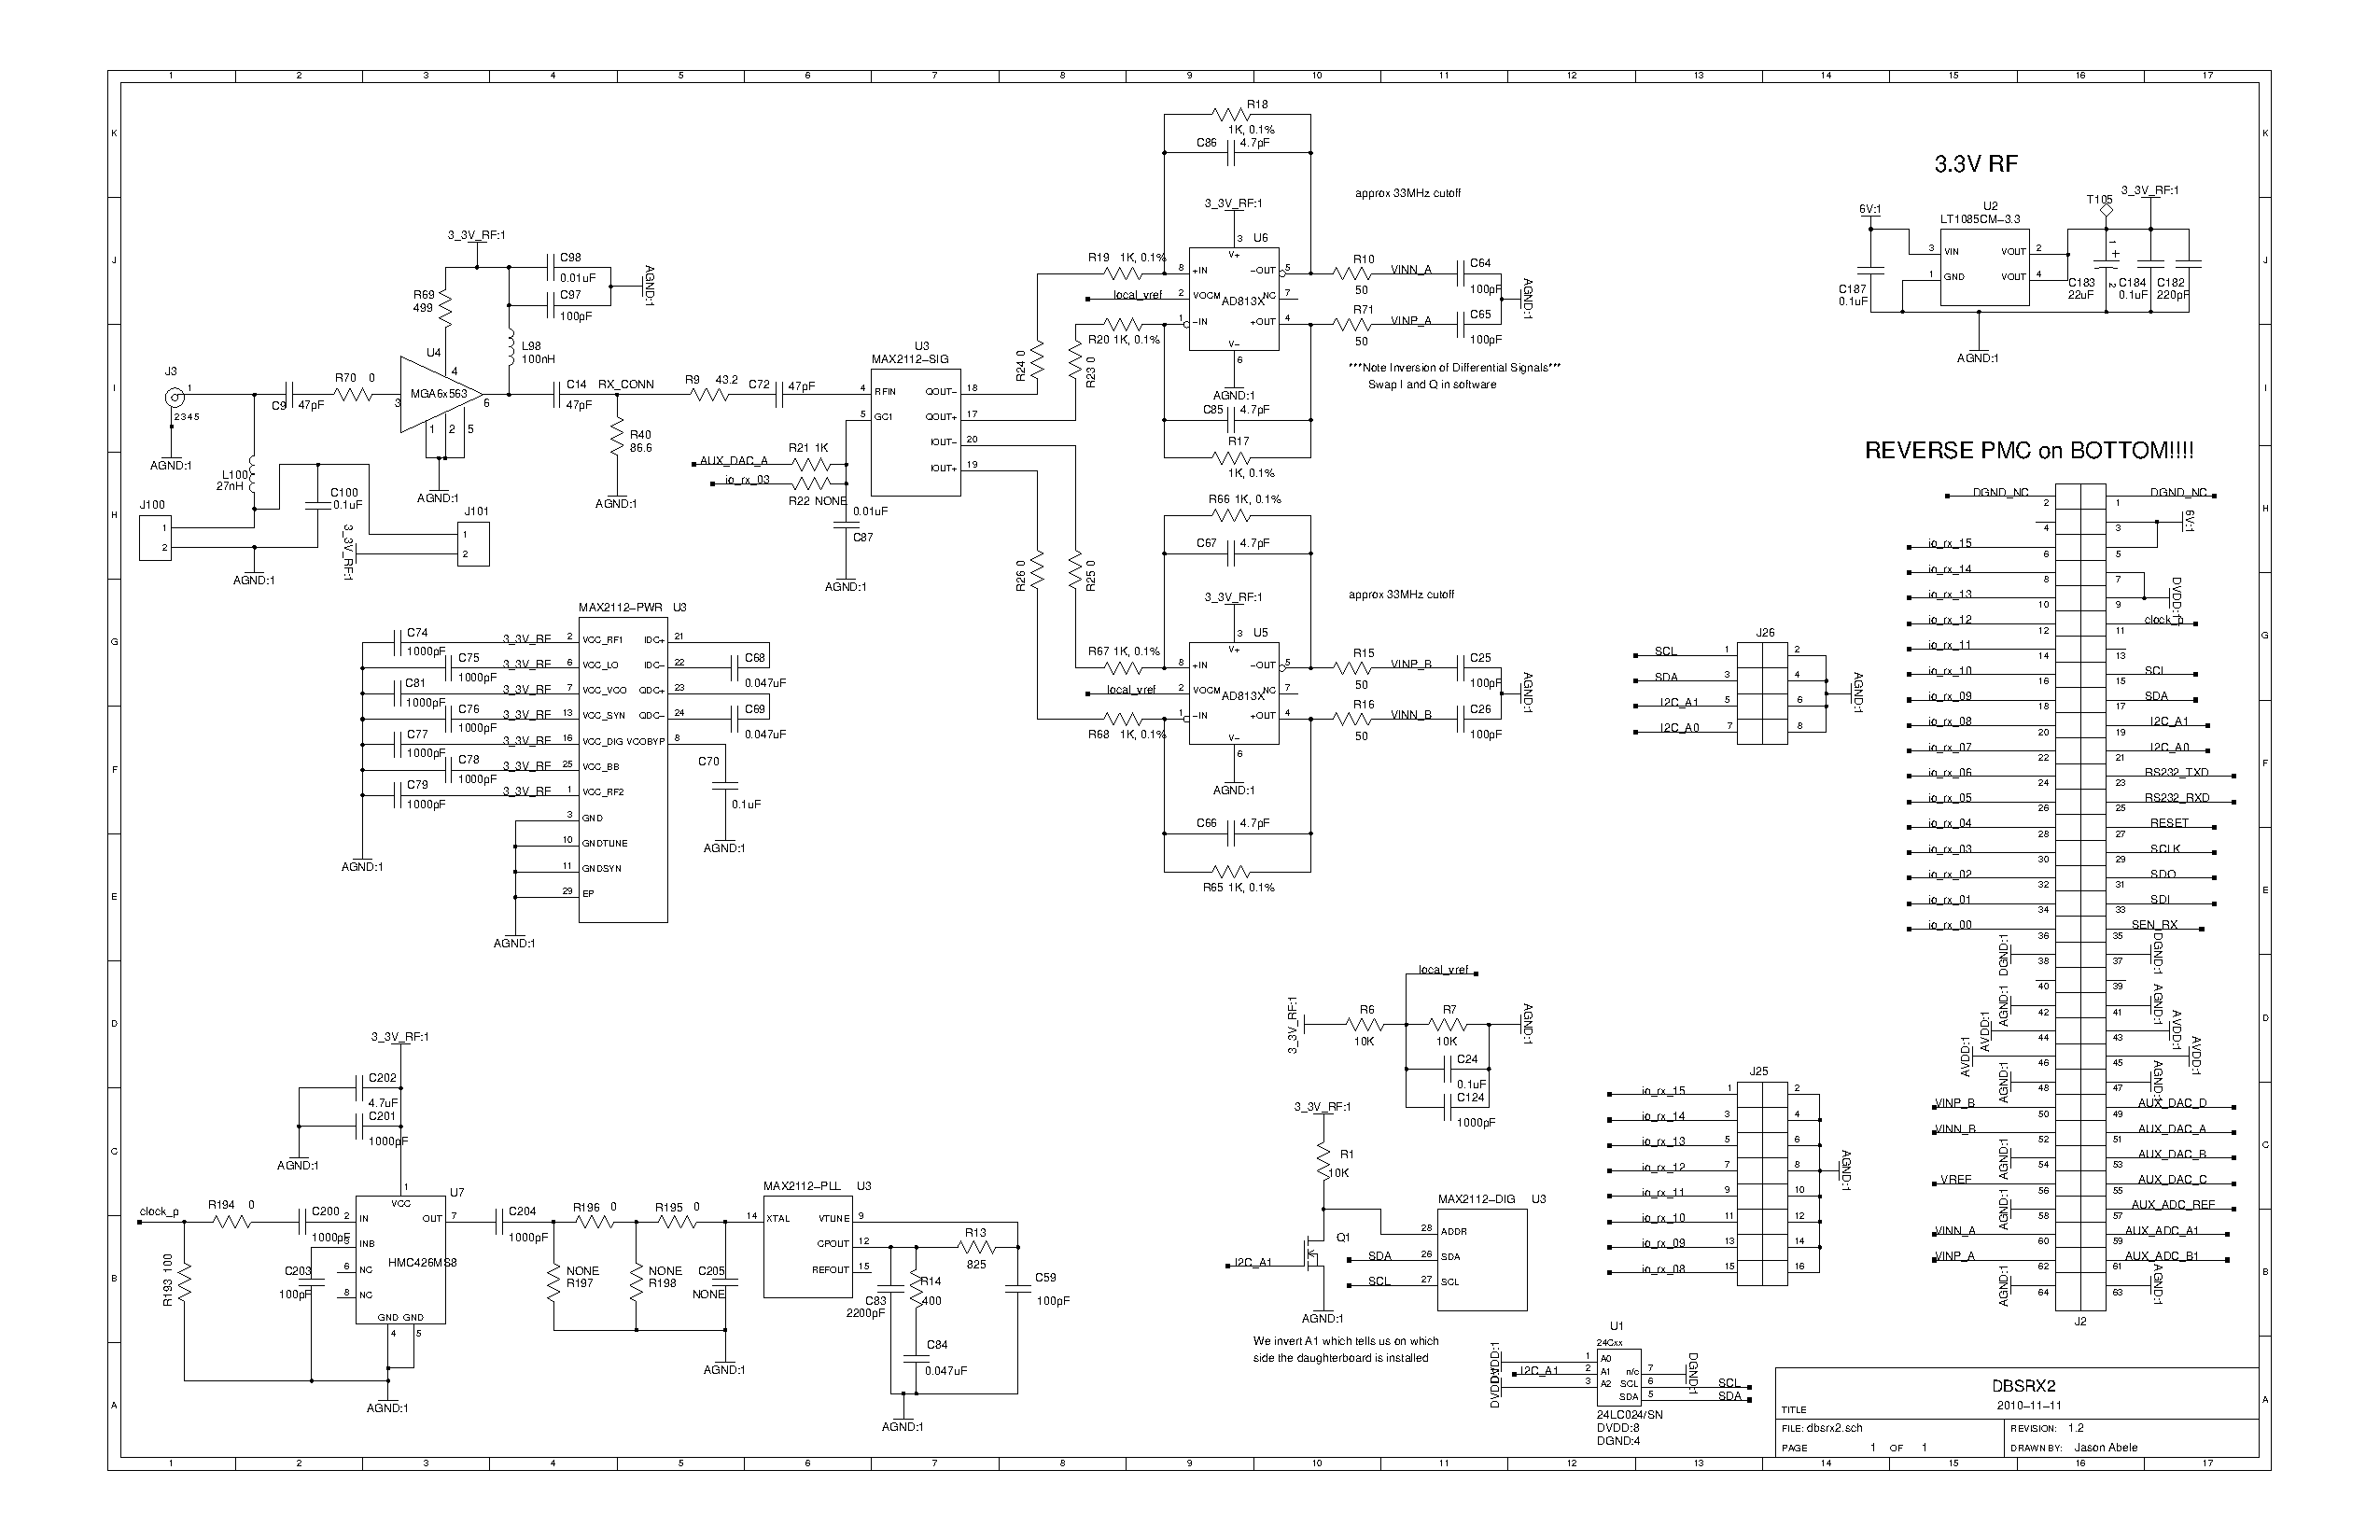
\includegraphics[width=\textwidth]{Images/dbsrx2.pdf}
%\isucaption{The DBSRX2 Schematic (Image from Ettus Research Website - www.ettus.com)}
%\label{dbsrx2_sch}
%\end{figure}
%}

These analog I and Q values are then sent to the analog to digital converter to be digitized.  The IQ values are transmitted as differential signals to minimize noise.  Once digitized, the digital I Q values are sent to a FPGA to be processed, and then sent to the PC for soft-ware based signal processing.

%Since we are using the DBSRX2 after the LNAs that are already in use, the noise temperature added by the DBSRX2 will be small.  The DBSRX2 adds approximately 1.05 dB to the overall noise factor of the system.

\subsection{Software Platform} \label{software_platform}

There are two pieces of software that are used with the software defined radio:  1) the firmware that is used in the FPGA of the N200, and 2) the software running on the host PC.  

The firmware provides low level processing of the signal before being sent to the software located on the PC.  It also provides a link for controlling key aspects of the software defined radio, such as gain, bandwidth and the center frequency.  This firmware comes pre-loaded into the FPGA by Ettus Research, and can be upgraded using tools provided by Ettus Research.

The software on the host PC performs signal processing on the I/Q data.  GNURadio was selected to be this software.   GNUradio is an open source software package designed for software defined radio application development.  It provides a GUI framework to create an interactive environment for the user, and is well supported by the N200 hardware.  

GNURadio uses a combination of Python and C++, where Python handles the high level interface and C++ is used to implement drivers and low level interfaces to the hardware.  This combination allows for a system that is easy to use, but still meets the demanding performance required for handling large amounts of data. 

GNURadio also has a rapid development tool called GNURadio companion (GRC).  GRC is a simple to use graphical system for designing and building radio components in software. An example of GRC is shown in figure \ref{N200_GRC}.

{\begin{figure}[h!tb] \centering
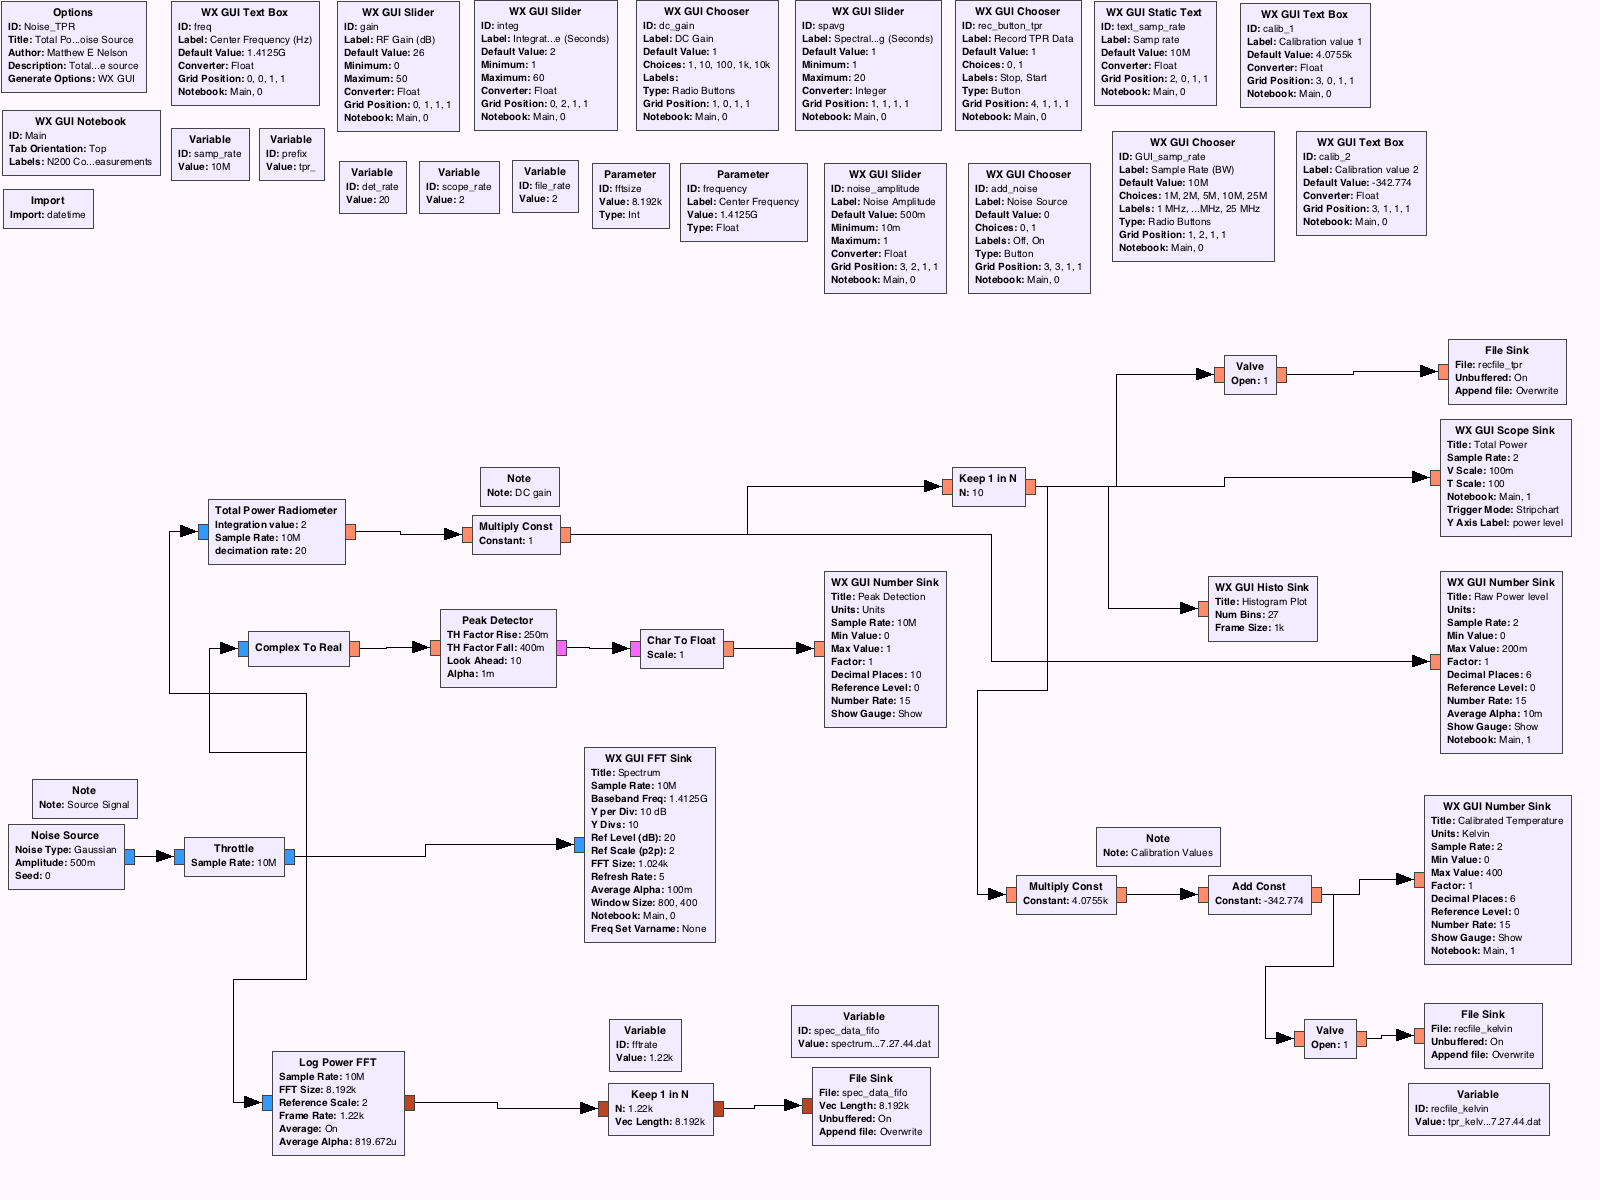
\includegraphics[width=\textwidth]{Images/noisesrc_radiometer.png}
\isucaption{A screenshot of the GNURadio Companion editor program.  Source:  GNURadio}
\label{N200_GRC}
\end{figure}
}

GNUradio Companion provides common functions, such as signal sources, signal processing and signal sinks, as blocks that can picked and placed on the screen.  Once placed, the blocks can be wired up, much like LabView, and the flow of data can be controlled in this fashion.  GNURadio Companion also includes blocks that allow for building a GUI interface, which can be used to display data and control the software defined radio.

If a block does not exist, it can be created.  Because GNURadio uses Python, users can use this powerful and flexible language to build new blocks that can be imported into GRC.  

%Additional blocks can also be created using Python.  This allows the users to create other blocks and access other common Python libraries.  Each block is then defined in While GNURadio Companion provides most of the essential blocks used in most applications additional blocks can by added if needed.  This is done by using Python and the blocks in GNUradio Companion are simply blocks of Python code.  To compile a GNURadio Companion flow diagram, you simply run the sheet, which then generates the Python code that is then executed.   


Using GNURadio and GNURadio Companion, a software defined radio can be rapidly built with little programming experience.  The excellent support of the hardware selected, and the ease of use made it an ideal development tool for building the necessary software for our software defined radiometer.

%----------------------------------------------------------
% End of Chapter 3.  Anything below this is extra information

%\subsection{Integration and filtering}\label{int_filt}

%Filtering with a traditional radiometer is usually accomplished by using mechanical filters.  Often these are band-pass filters that limit the bandwidth that the radiometer sees.  Other filters, such as a low pass filter are also used, but usually to smooth out the output from the square law detector.  Another item used to help smooth out the signal from the square law detector is an integrator.

%In a traditional radiometer, we can integrate by using a simple RC circuit, which consists of a resistor and capacitor.  To begin, we will examine how a RC filter is analogous to an integrator where the R and C values determine our time constant and our integration time for the filter[\cite{Aitken}].  We know a RC filter is analogous to an integrator by looking at equation \ref{eq:rc_int}.  

%\begin{equation}\label{eq:rc_int}
%\frac{1}{RC}\int{V_idt}
%\end{equation}

%To begin with, we look at what an analog RC filter looks like. 

%{\begin{figure}[h!tb] 
%\centering
%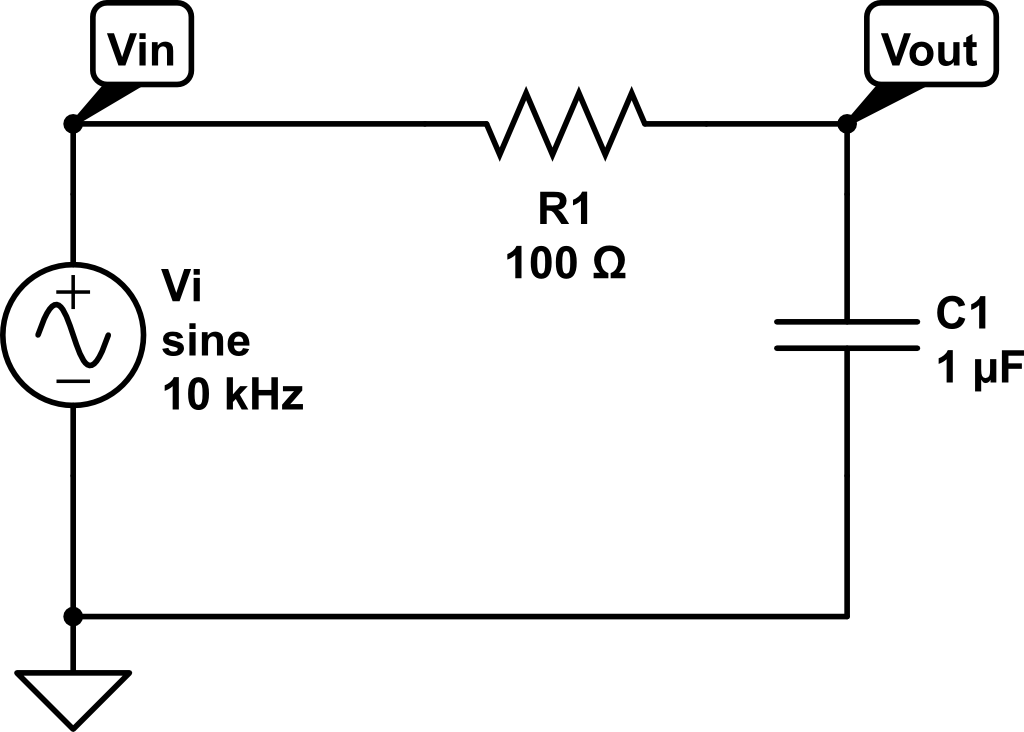
\includegraphics[width=10cm]{Images/rc-circuit.png}
%\isucaption{A simple RC circuit}
%\label{rc_circuit}
%\end{figure}
%}

%This circuit can be represented by equation \ref{eq:rc_circuit_eq}.

%\begin{equation}\label{eq:rc_circuit_eq}
%\frac{V_{in}-V_{out}}{R}=C\frac{dV_{out}}{dt}
%\end{equation}

%For the cutoff frequency of a RC circuit, we know that it has the relationship shown in equation \ref{RC_relationship}.

%\begin{equation}\label{RC_relationship}
%f_c=\frac{\sqrt{3}}{2\pi RC}\rightarrow RC=\frac{\sqrt{3}}{2\pi f_c}
%\end{equation}

%The $RC$ term gives us our time constant of the circuit and can be used to calculate out our coefficients. 


%The RF front end plays an important role in the radiometer because the LNAs used in the front end have a large impact on the system noise generated by the radiometer itself.  A traditional radiometer utilizes both amplification through the LNAs and also includes filtering to the desired bandwidth.  A SDR radiometer does not require the filters as we are able to create these in software, however the amplification stages need to remain.  

%{\begin{figure}[h!tb] 
%\centering
%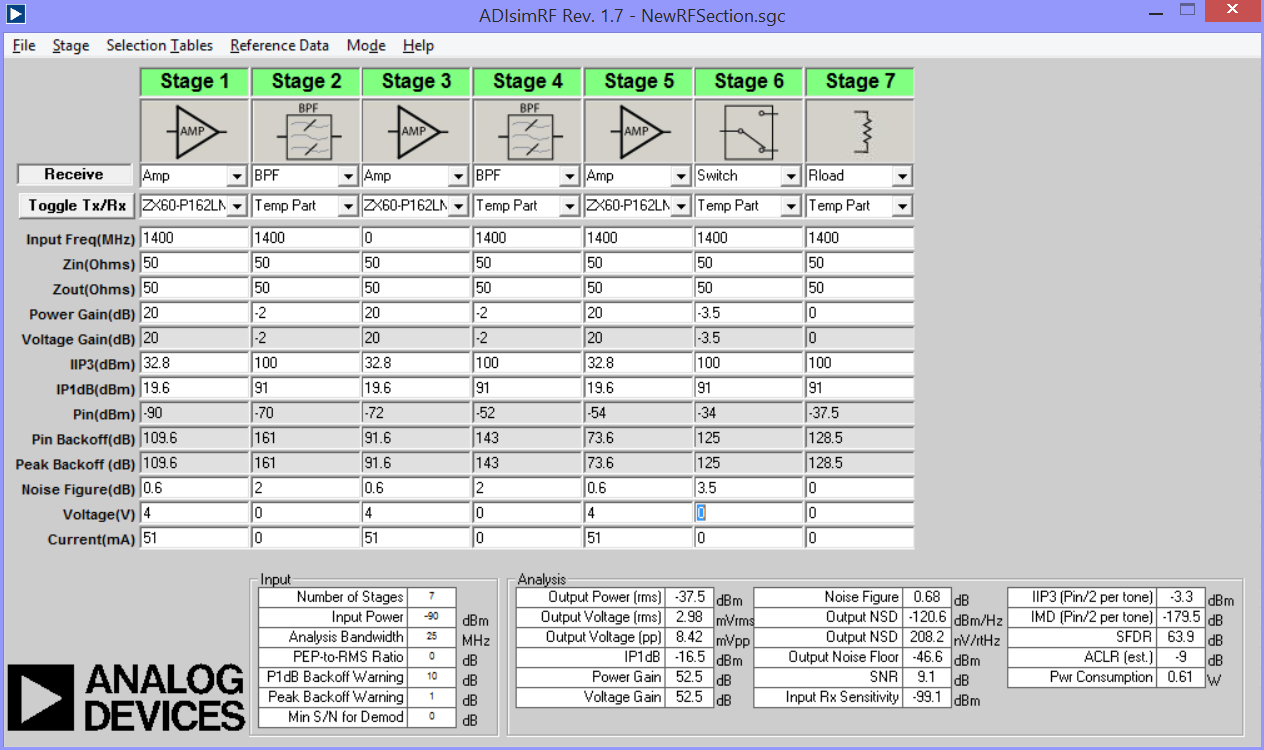
\includegraphics[width=0.8\linewidth]{Images/RF_Front_end.png}
%\isucaption{The ADISIMRF program used to verify the design of the RF Front End}
%\label{ISU_Rad}
%\end{figure}
%}

%A typical RF front end uses a two to four stage Low Noise Amplifier (LNA) to amplifier the noise while keeping the noise contributed to the system as low as possible.  As with any radiometer, the first LNA is the most critical as it contributes the most to the overall system noise temperature.  For this reason a LNA that did not have a large gain but had a low noise figure is chosen. The second and third LNA has higher gain values at the cost of a higher noise figure, although not by much.  However, since they are further down the chain, they do not contribute as much to the total system noise.  


%The amount of noise that is generated by the object of interest is due to the thermal agitation of the charge carriers, usually the electrons, which is directly correlated to the physical temperature of the source[\cite{Nyquist1928thermal}].  This correlation is done as a noise temperature.  All objects emit this noise and the intensity will vary on multiple parameters and on what the source is.  One source that has current research at Iowa State University is in detecting soil moisture.  Numerous soil types can be observed including sandy types of soil[\cite{Liu}], The brighter or warmer the noise temperature is, the more RF noise that has been received which correlates to a drier soil.  The less RF noise power received the cooler the noise temperature and this indicates wetter soil area. Radiometers such as these are already in service on satellites such as the Soil Moisture and Ocean Salinity (SMOS) satellite launched by the European Space Agency (ESA) and are used by scientists to monitor the Earth's soil moisture and ocean salinity[[\cite{McMullan}][\cite{Hardy}]. 

%{\begin{figure}[h!tb] 
%\centering
%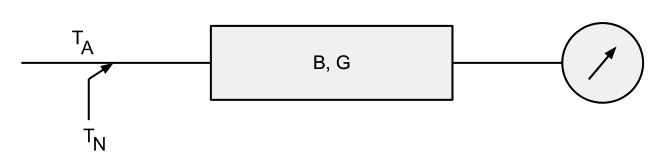
\includegraphics[width=\textwidth]{Images/radiometer_noise_added.png}
%\isucaption{A more realistic radiometer model}
%\label{noiserad}
%\end{figure}
%} 

%{\begin{figure}[h!tb] 
%\centering
%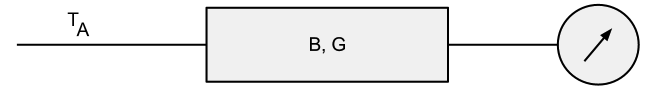
\includegraphics[width=\textwidth]{Images/simple_rad.png}
%\isucaption{The ideal radiometer block diagram}
%\label{simplerad}
%\end{figure}
%}

%Figure \ref{simplerad} shows us an ideal radiometer.  That is a radiometer that has an input from the antenna, $T_{A}$, a known bandwidth denoted as $B$ or $\beta$ and a known gain denoted as $G$.  At the end of the block is the detector, which measures the power from the radiometer.

%Only a certain selection of the radio spectrum is observed by the radiometer and this is the bandwidth of the radiometer.  In our scenario, we center around 1.4125 GHz.  There is a reason why 1.4125 GHz is selected and that is from 1.4000 to 1.4250 GHz is protected internationally to be as radio frequency interference free as possible.  This reduces interference from outside sources such as transmitters that can interfere with the operation of the radiometer.  

%The power coming from the antenna is the combination of the following items:

%\begin{enumerate}
%\item Gain or $G$ of the system,
%\item Bandwidth or $\beta$ of the system,
%\item Signal source or $T_{A}$.
%\end{enumerate}

%These specifications had a large impact on the selection of the N200 for this application.  Specifically the 14-bit ADC, the 50 MS/s and the modular daughter-board system were the largest factors in the decision to use the N200 SDR.  Further explanation on these specifications are explained in the following sections.

%\emph{14-bit ADC.}  The analog to digital converters (ADC) allow us to take the analog I and Q values from the daughter boards and digitize this information.  Once digitized, we can now work with the signal both on the on-board FPGA board or stream it to the computer so that our software can manipulate the signal.  In radiometry, we are primarily looking at the overall power of the signal and this does not require us to accurately recreate the signal.  However, as will discuss later there are times were we do want frequency information and having an accurate frequency representation of the signal will then be an important factor.

%\emph{50 MS/s Bandwidth.}  The N200 is capable of working with up to 100 MS/s signal and can stream up to 50 MS/s through the Gigabit Ethernet connection.  The N200 also has the ability to have up to 2 daughter boards installed.  If we assume each will have up to a 20 MHz signal, this means up to 40 MS/s of data will be required.  This means that the N200 meets and can exceed the bandwidth requirements that we were looking for.  In addition, the FPGA on the N200 is capable of working with up to 100 MS/s, so there is room in handling additional bandwidth by using the on board FPGA to process the signal.

%The daughter board selected is the DBSRX2 card as this card is receive only and operates between 800 MHz and 2.4 GHz.  The DBSRX2 also has built in amplification that is adjustable through software.

%{\begin{figure}[h!tb] 
%\centering
%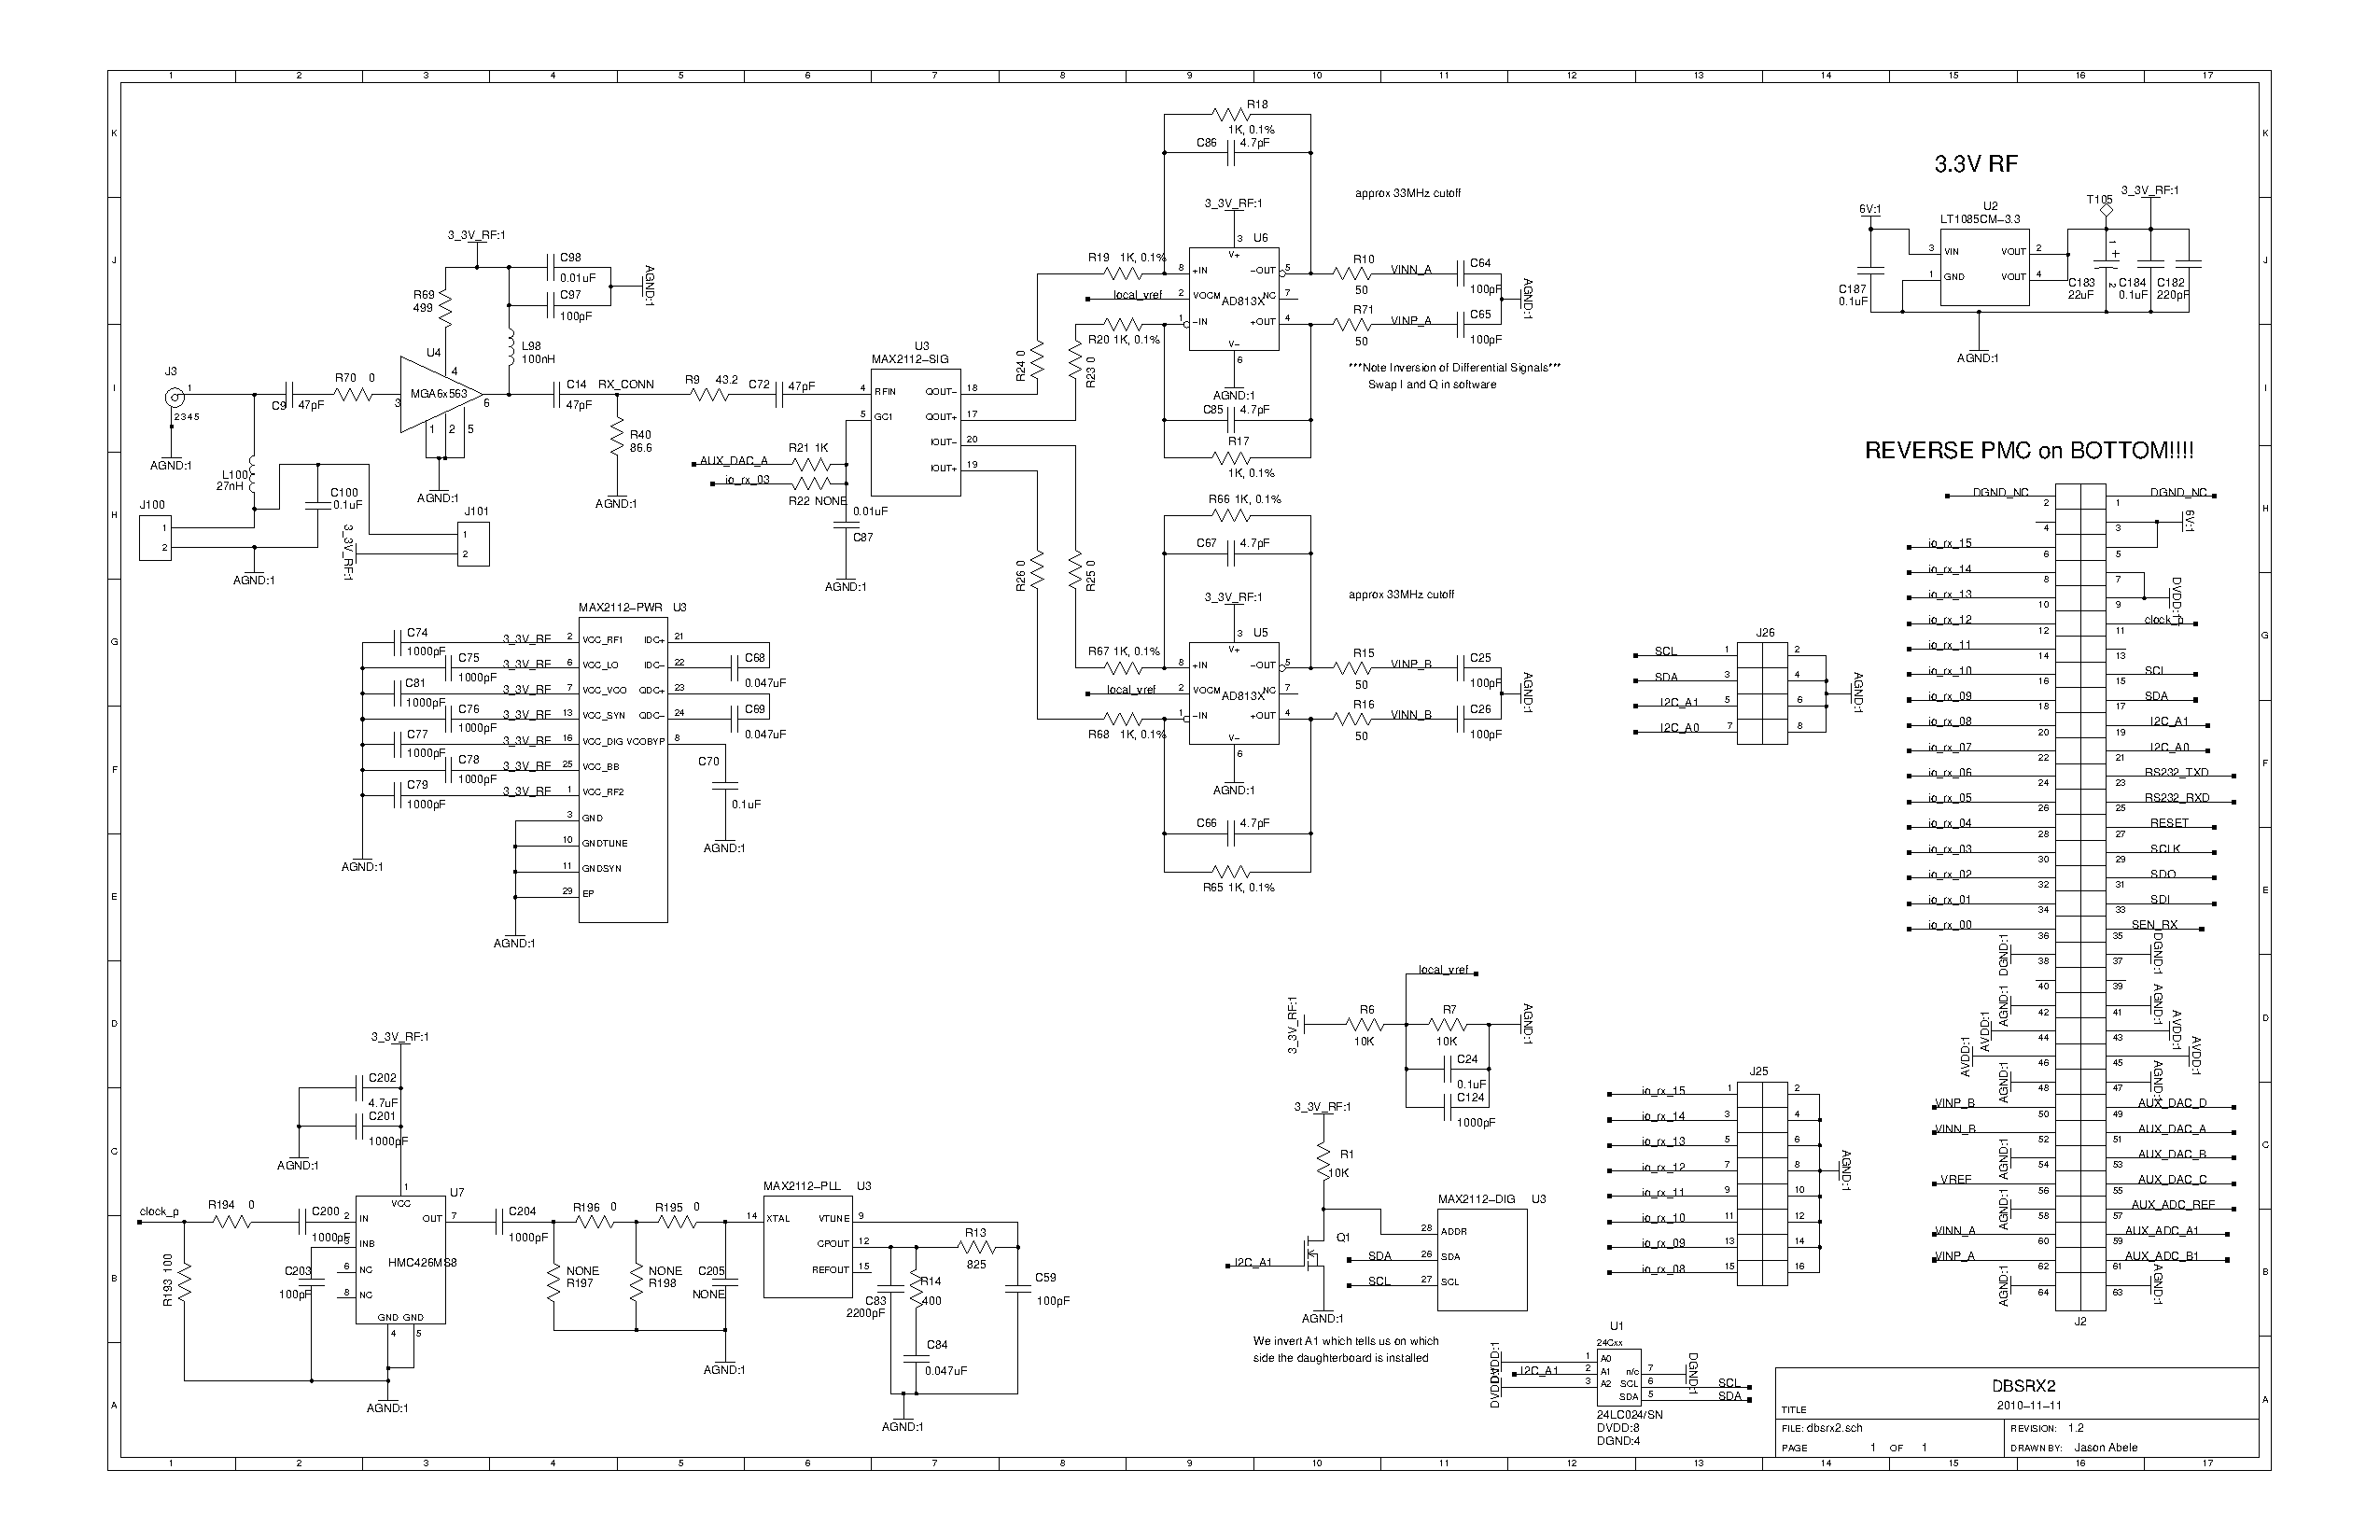
\includegraphics[width=\textwidth]{Images/dbsrx2.pdf}
%\isucaption{The DBSRX2 Schematic (Image from Ettus Research Website - www.ettus.com)}
%\label{dbsrx2_sch}
%\end{figure}
%}

%GNURadio  and GRC is written in Python, which allows for easy modification and access to additional tools that can be used with GNURadio.  While most of GNURadio is written in Python, C is used for any of the low level drivers and interface to the hardware.  This is done to optimize speed and performance of GNURadio.

%GNURadio fills in the software side of the software defined radio.  Although there is firmware that runs on the FPGA in the N200, this firmware is designed to communicate with a host PC.  It is this software that does most of the work by doing the calculations that apply to the signal.  The FPGA simply sends the raw IQ data to the host PC, which then performs the necessary math functions.  Again, the reason why software defined radios are desirable is the ability to change the behavior of the radio quickly.  In our scenario we can change functionality by simply loading a new software program in the host PC.  

%This functionality is ideal for communication type of radios where different modulation schemes and encoding and decoding methods can easily be changed out.  However, in a radiometer we are not interested in this aspect of the SDR.  However, one functionality is available that can be valuable for a radiometer, and that is with filtering.  Although we often use frequencies that should be free from interference, this is not always what happens in the real world.  Interference can and often does still occur, even in these protected frequencies.  With the SDR, we are able to quickly adapt to changing conditions by moving the frequency, changing our bandwidth and even filter out an offending signal.  

%GNURadio was selected as it is an open source software platform.  GNURadio is licensed under the GPL license and has a strong community that continually updates the software.  It is also well supported by third parties such as Ettus Research Group, National Instruments and other SDR developers.  In addition, GNURadio has a strong set of tools that can be used to develop programs that run under GNURadio.  Tools such as the GNURadio Companion (GRC) allows for an easy to use GUI to develop code for GNURadio.  GNURadio is also written in Python, which allows for easy modification and access to additional tools that can be used with GNURadio. 

%{\begin{figure}[h!tb] 
%\centering
%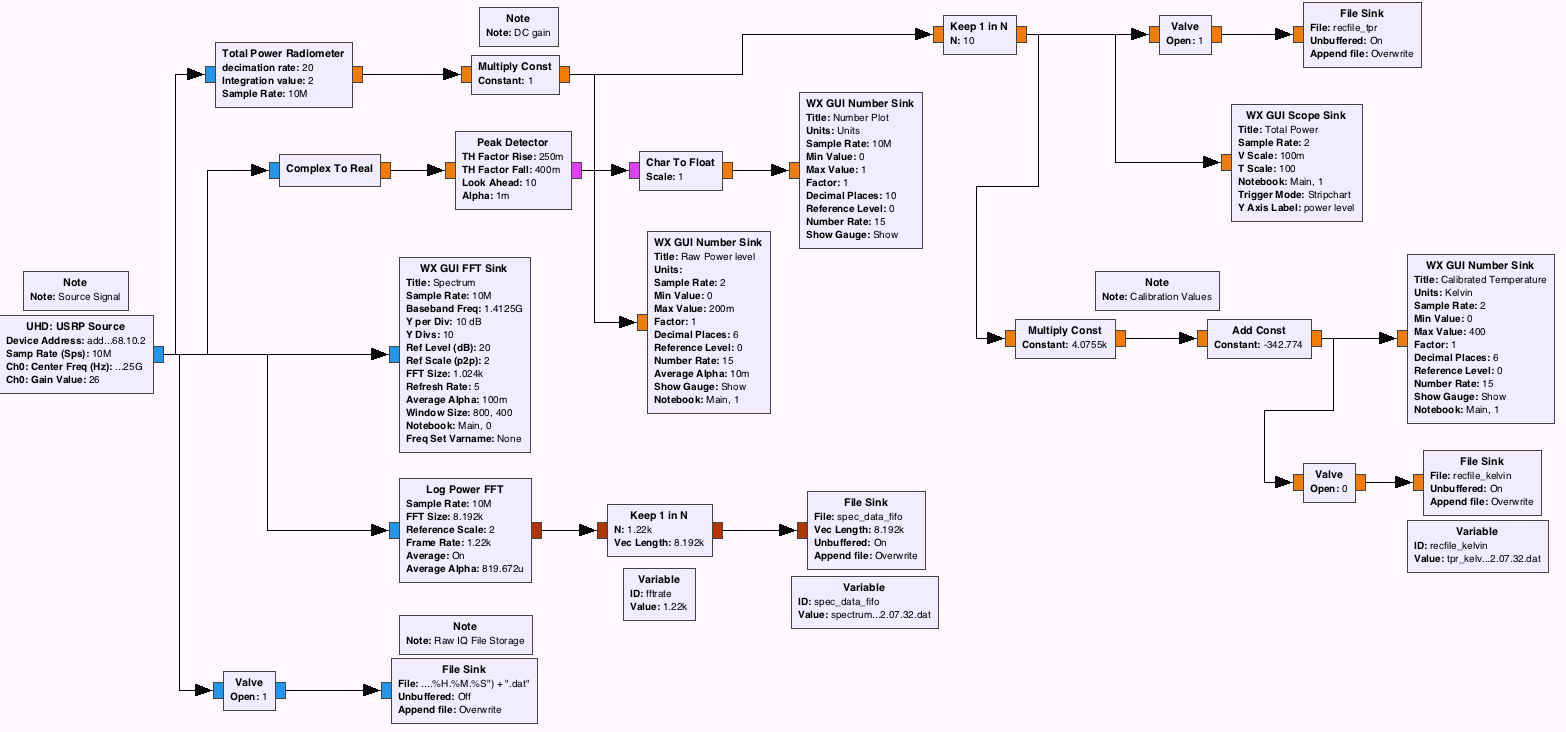
\includegraphics[width=17cm]{Images/N200_radiometer_grc.png}
%\isucaption{Screenshot of the GNURadio Companion editor and the N200 Radiometer block diagram used in the author's experiments}
%\label{N200_GRC}
%\end{figure}
%}
 